\chapter{Propuesta de solución}
\label{chap:chapter2}

\section*{Introducción}
\addcontentsline{toc}{section}{Introducción}
Este capítulo presenta la propuesta de solución para abordar el problema identificado en la investigación: la interpretación y contextualización de datos no estructurados del transporte marítimo extraídos del Diario de la Marina (1844–1960). Aquí se detallan los requisitos funcionales (RF) y no funcionales (RNF) que el sistema debe cumplir, así como una descripción exhaustiva de la solución propuesta, incluyendo las historias de usuario y las tarjetas CRC (Clase-Responsabilidad-Colaboración). Además, se analizan los patrones arquitectónicos y de diseño seleccionados para estructurar la aplicación, junto con las buenas prácticas de codificación asociadas a las tecnologías empleadas. Finalmente, se incluyen el diagrama de clases y el diagrama de componentes, que ilustran los elementos clave que integran esta propuesta. Este capítulo sienta las bases técnicas y conceptuales para la implementación y validación descritas en capítulos posteriores, alineándose con los objetivos específicos de diseño e implementación establecidos en la introducción.

\section{Descripción de la Propuesta de Solución}
\label{sec:propuesta_solucion}

La solución propuesta aborda la interacción con los datos históricos del transporte marítimo del \textit{Diario de la Marina} (1844-1960) mediante el desarrollo de una aplicación web moderna, separando claramente las responsabilidades entre la interfaz de usuario, la lógica de negocio y el procesamiento avanzado de lenguaje natural. Esta arquitectura se compone de tres elementos principales: un \textit{frontend} desarrollado con \textbf{React js}, un \textit{backend} API construido con \textbf{Django REST Framework}, y un microservicio dedicado que alberga el \textbf{sistema multiagente conversacional} basado en inteligencia artificial y que se expone con una api creada con \textbf{FastApi}. Esta elección arquitectónica promueve la escalabilidad, la mantenibilidad y la separación de intereses, permitiendo que cada componente evolucione de forma independiente.

% Incluye aquí tu nueva figura de arquitectura web
\begin{figure}[htbp] % h: here, t: top, b: bottom, p: page of floats - ajusta según necesidad
	\centering
	% Asegúrate de que la ruta 'images/arquitectura_web.png' sea correcta
	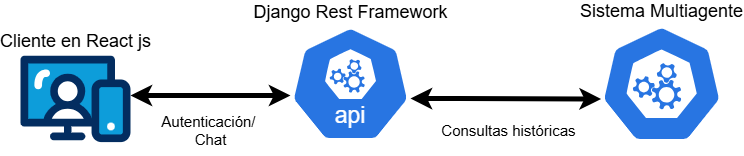
\includegraphics[width=0.9\textwidth]{images/micro.png} 
	\caption{Arquitectura de la propuesta de solución.}
	\label{fig:arquitectura_web}
\end{figure}

La Figura \ref{fig:arquitectura_web} ilustra la arquitectura general. El flujo de interacción del usuario es el siguiente:

\begin{enumerate}
	\item El usuario interactúa con la interfaz web desarrollada en \textbf{React}, donde ingresa sus consultas en lenguaje natural (e.g., “¿Qué barcos llegaron de Europa en enero de 1850?”).
	\item El frontend React envía la consulta del usuario, típicamente como una petición HTTP (e.g., POST con JSON), al \textit{endpoint} correspondiente del \textbf{backend DRF}.
	\item El backend DRF actúa como orquestador principal de la lógica de negocio. Puede gestionar autenticación de usuarios (si aplica), almacenar historial de conversaciones, y, crucialmente, procesa la solicitud entrante. Determina que la consulta requiere procesamiento por IA y la reenvía al \textbf{microservicio del MAS} a través de una llamada API interna (e.g., HTTP/JSON o gRPC).
	\item El \textbf{microservicio MAS} recibe la consulta y ejecuta su lógica interna basada en agentes para procesar el lenguaje natural, buscar en la base de datos vectorial del \textit{Diario de la Marina}, contextualizar la información y generar la respuesta (texto y/o imágenes).
	\item El microservicio MAS devuelve el resultado procesado (e.g., un objeto JSON con texto y/o datos de imagen) al backend DRF.
	\item El backend DRF recibe la respuesta del microservicio, la formatea si es necesario (e.g., preparándola para la visualización), y la envía de vuelta al frontend React.
	\item Finalmente, el frontend \textbf{React} recibe la respuesta del backend y la presenta al usuario de forma clara y ordenada en la interfaz de chat, mostrando el texto y/o las imágenes generadas.
\end{enumerate}

Dentro del \textbf{microservicio del MAS} opera la lógica conversacional avanzada, cuyo flujo interno se detalla a continuación y se ilustra en la Figura \ref{fig:flujo_mas_interno}. Este microservicio está diseñado específicamente para transformar los datos históricos no estructurados en conocimiento estructurado y accesible, superando las limitaciones de herramientas previas mediante la integración de LLMs, RAG y una coordinación eficiente entre agentes especializados.

% Renombra la etiqueta de tu figura original y ajusta la referencia
\begin{figure}[htbp] 
	\centering
	% Asegúrate de que la ruta 'images/mas.png' sea correcta
	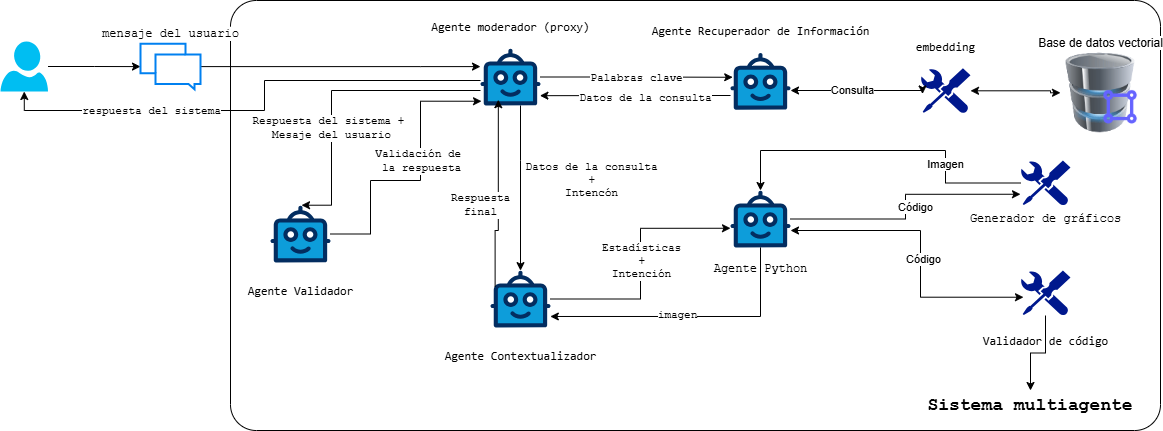
\includegraphics[width=1\textwidth]{images/mas.png} 
	\caption{Flujo Interno del Microservicio Multiagente Conversacional.}
	\label{fig:flujo_mas_interno} % Nueva etiqueta para la figura original
\end{figure}

El proceso interno del microservicio (Figura \ref{fig:flujo_mas_interno}) inicia cuando recibe una consulta del backend DRF. Esta consulta es manejada por el \textbf{Agente de Moderación (proxy)}, que actúa como coordinador central dentro del microservicio. Este agente extrae palabras clave (e.g., “barcos”, “Europa”, “enero 1850”) y determina la intención del usuario. A continuación, delega la tarea al \textbf{Agente Recuperador de Información}, que convierte las palabras clave en embeddings y consulta la base de datos vectorial especializada para recuperar fragmentos relevantes del \textit{Diario de la Marina}. Los datos recuperados se devuelven al Agente de Moderación. Posteriormente, el Agente de Moderación envía la información recuperada, junto con la intención, al \textbf{Agente Contextualizador}. Este agente evalúa si se necesita una respuesta textual, estadísticas gráficas o ambas. Si se requieren gráficos (e.g., un gráfico de la frecuencia de llegada de barcos por mes), genera instrucciones que se envían al \textbf{Agente Python}. Este agente crea un script Python para generar la visualización, valida su corrección y lo convierte en una imagen. La imagen resultante se retorna al Agente Contextualizador. Si no se requieren gráficos, el Agente Contextualizador enriquece la información textual con contexto histórico relevante usando técnicas RAG. Antes de enviar la respuesta final de vuelta al backend DRF, el \textbf{Agente Validación} revisa la coherencia y precisión del contenido generado (texto y/o imagen), comparándolo con la consulta original. Finalmente, el Agente de Moderación ensambla la respuesta validada y la retorna como salida del microservicio. 

Esta arquitectura desacoplada, combinando una interfaz web moderna, un backend robusto y un microservicio especializado en IA, no solo facilita la interacción del usuario y la gestión de datos, sino que también optimiza la investigación histórica, contribuye a la preservación del patrimonio documental y permite escalar los componentes de IA de forma independiente.


\section{Análisis de requisitos}

El análisis de requisitos da como resultado la especificación de las características operativas del software. Indica la interfaz de este y otros elementos del sistema, y establece las restricciones que limitan al software \cite{pressman2010practitioner}.Es una fase crucial en el proceso de desarrollo de software. Se trata de una etapa inicial en la cual un analista busca entender las necesidades del cliente y traducirlas en un conjunto de requisitos claros y bien definidos \cite{palli2023analisis}.

\subsection{Técnicas de captura de requisitos}


La definición de los requisitos del sistema se fundamenta en un proceso sistemático de captura, basado en dos técnicas ampliamente reconocidas en ingeniería de software: la entrevista y la observación, aplicadas en el contexto de los ejemplos analizados en el estado del arte (Capítulo 1). Estas técnicas, permitieron identificar las expectativas de los usuarios potenciales y las limitaciones de las soluciones existentes, asegurando que los requisitos reflejen tanto las demandas prácticas como las carencias técnicas observadas~\cite{sommerville2011software}.

\textbf{Entrevista:} Se realizaron entrevistas semiestructuradas con historiadores y académicos especializados en historia del Caribe, quienes serían usuarios finales del sistema. Las preguntas se diseñaron para explorar sus necesidades al interactuar con documentos históricos digitalizados, como el \textit{Diario de la Marina}. Por ejemplo, se les consultó: ``¿Qué tipo de información busca con mayor frecuencia en archivos históricos?'' y ``¿Qué dificultades encuentra al analizar datos marítimos de textos antiguos?''. Las respuestas destacaron la importancia de obtener respuestas contextualizadas (e.g., vinculadas a eventos históricos), la necesidad de visualizaciones gráficas para patrones comerciales y la frustración con errores de transcripción que dificultan el análisis. Estas aportaciones guiaron la definición de requisitos como la corrección de datos y la generación de gráficos.

\textbf{Observación:} Se analizaron las plataformas del estado del arte (LangChain, Chatize, Haystack) mediante una observación activa de su funcionamiento con documentos de prueba, incluyendo algunos fragmentos digitalizados del \textit{Diario de la Marina}. Este proceso consistió en interactuar con las herramientas, registrar sus respuestas a consultas simuladas (e.g., ``Lista de puertos en 1850'') y evaluar su desempeño en términos de precisión, contextualización y usabilidad. Los resultados revelaron que, aunque estas soluciones manejan bien textos modernos, fallan en interpretar correctamente términos arcaicos, no integran contexto histórico externo y carecen de capacidades gráficas avanzadas \cite{lewis2020retrieval, langchain2023}. Estas observaciones subrayaron la necesidad de un sistema más especializado, con agentes dedicados a la contextualización y visualización.

La combinación de entrevistas y observación permitió triangular las necesidades de los usuarios con las deficiencias técnicas de las soluciones actuales, proporcionando una base sólida para los requisitos funcionales y no funcionales que se detallan a continuación.



\subsection{Requisitos funcionales}

Los requisitos funcionales son enunciados acerca de servicios que el sistema debe proveer, de cómo debería reaccionar a entradas particulares y de cómo debería comportarse en situaciones específicas \cite{sommerville2011software}. Estos requisitos describen tanto las interacciones previstas entre el software y su entorno, como las funcionalidades y servicios que el sistema debe proporcionar a los usuarios. Además, son recopilados y documentados durante el proceso de análisis de negocio y se convierten en una parte fundamental del contrato de desarrollo de software. Pueden incluir, por ejemplo, la capacidad de un sistema para permitir a los usuarios adjuntar un archivo, eliminar o editar un elemento seleccionado, así como la forma en que el sistema debe reaccionar a ciertas entradas o situaciones particulares \cite{chanchi2019propuesta}.

A continuación, se describen los requisitos funcionales específicos para el sistema multiagente conversacional propuesto:

\begin{longtable}{@{}l >{\raggedright\arraybackslash}p{4.5cm} >{\raggedright\arraybackslash}p{6.5cm} l l@{}} % Ajustados anchos
	\caption{Tabla de Requisitos Funcionales (RF)} \label{tab:requisitos_funcionales_final} \\ 
	\toprule
	\textbf{ID} & \textbf{Nombre} & \textbf{Descripción} & \textbf{Complejidad} & \textbf{Prioridad} \\ 
	\midrule
	\endfirsthead 
	
	\caption[]{Tabla de Requisitos Funcionales (RF) (Continuación)} \\ 
	\toprule
	\textbf{ID} & \textbf{Nombre} & \textbf{Descripción} & \textbf{Complejidad} & \textbf{Prioridad} \\ 
	\midrule
	\endhead 
	
	\bottomrule
	\multicolumn{5}{r@{}}{\textit{Continúa en la siguiente página...}} \\ 
	\endfoot 
	
	\bottomrule
	\endlastfoot 
	
	% --- Gestión de Usuarios y Autenticación ---
	\textbf{RF1} & Registrar nuevo usuario & Permitir a un visitante registrarse proporcionando datos válidos (e.g., email, contraseña), que serán almacenados de forma segura por el backend. & Media & Alta \\ 
	\textbf{RF2} & Autenticar usuario existente & Permitir a un usuario registrado iniciar sesión proporcionando credenciales válidas, verificadas por el backend, generando una sesión activa. & Media & Alta \\ 
	\textbf{RF3} & Cerrar sesión de usuario & Permitir al usuario autenticado finalizar su sesión activa en el sistema. & Baja & Media \\ 
	\textbf{RF4} & Proteger acceso a funcionalidades & Asegurar que solo los usuarios autenticados puedan acceder a las funcionalidades de chat, historial y consulta de datos históricos. & Media & Alta \\ 
	% --- Gestión de Conversaciones ---
	\textbf{RF5} & Iniciar nueva conversación & Permitir al usuario autenticado crear una nueva sesión de chat independiente de las anteriores. & Baja & Alta \\ % NUEVO
	\textbf{RF6} & Listar conversaciones anteriores & Mostrar al usuario autenticado una lista de sus conversaciones previas para poder seleccionarlas y revisarlas. & Media & Media \\ % NUEVO
	\textbf{RF7} & Seleccionar conversación existente & Permitir al usuario seleccionar una conversación de su historial para visualizarla y continuarla. & Media & Media \\ % NUEVO
	\textbf{RF8} & Eliminar conversación del historial & Permitir al usuario eliminar permanentemente una conversación específica de su historial. & Media & Baja \\ % NUEVO
	\textbf{RF9} & Persistir historial de conversaciones & El backend debe almacenar de forma persistente las consultas y respuestas asociadas a cada conversación de cada usuario. & Media & Alta \\ % NUEVO (Lógica Backend)
	% --- Interfaz y Flujo del Chat ---
	\textbf{RF10} & Ingresar consulta en chat activo & Permitir al usuario escribir y enviar una consulta en lenguaje natural dentro de la conversación activa. & Baja & Alta \\ 
	\textbf{RF11} & Visualizar intercambio en chat & Mostrar de forma clara y ordenada el diálogo (consultas del usuario y respuestas del sistema) dentro de la conversación activa. & Media & Alta \\ 
	\textbf{RF12} & Limpiar contenido del chat actual & Permitir al usuario borrar visualmente el contenido de la conversación activa en la interfaz (sin eliminarla del historial). & Baja & Baja \\ 
	\textbf{RF13} & Transmitir consulta al backend & El frontend debe enviar la consulta del usuario, junto con el identificador de la conversación activa y el token de sesión, al backend. & Media & Alta \\ 
	\textbf{RF14} & Recibir consulta y contexto & El backend debe recibir la consulta, el ID de conversación y validar la sesión antes de procesar la solicitud. & Media & Alta \\ 
	\textbf{RF15} & Delegar procesamiento de consulta al MAS & El backend debe enviar la consulta (y potencialmente contexto de conversación si es relevante para el MAS) al microservicio MAS para su procesamiento. & Media & Alta \\ 
	% --- Procesamiento Interno del Microservicio MAS ---
	\textbf{RF16} & Recibir solicitud de procesamiento & El microservicio MAS debe recibir la consulta (vía API) para iniciar el flujo de agentes. & Media & Alta \\ 
	\textbf{RF17} & Extraer palabras clave de consulta & El Agente Moderador debe analizar la consulta para identificar términos clave relevantes. & Alta & Alta \\ 
	\textbf{RF18} & Determinar intención de consulta & El Agente Moderador debe interpretar el propósito principal de la consulta del usuario (información, análisis, etc.). & Alta & Alta \\ 
	\textbf{RF19} & Generar embeddings para búsqueda & El Agente Recuperador debe convertir las palabras clave en representaciones vectoriales (embeddings) adecuadas para la búsqueda semántica. & Alta & Alta \\ 
	\textbf{RF20} & Recuperar información de BD Vectorial & El Agente Recuperador debe buscar y obtener fragmentos de texto relevantes del \textit{Diario de la Marina} desde la base de datos vectorial, basándose en los embeddings. & Alta & Alta \\ 
	\textbf{RF21} & Sintetizar y contextualizar respuesta textual & El Agente Contextualizador debe generar una respuesta coherente en lenguaje natural, integrando la información recuperada y añadiendo contexto histórico si es pertinente. & Alta & Alta \\ 
	\textbf{RF22} & Identificar necesidad de visualización & El Agente Contextualizador debe determinar si la consulta o los datos recuperados justifican la creación de una representación gráfica. & Media & Media \\ 
	\textbf{RF23} & Formular instrucciones para gráfico & Si se requiere un gráfico, el Agente Contextualizador debe generar las especificaciones (tipo de gráfico, datos a usar) para el Agente Python. & Alta & Alta \\ 
	\textbf{RF24} & Generar script de visualización & El Agente Python debe crear un script ejecutable (Python) que produzca la visualización solicitada a partir de los datos y especificaciones. & Alta & Alta \\ 
	\textbf{RF25} & Validar corrección de script & El Agente Python debe verificar que el script generado es sintácticamente correcto y no contiene errores obvios antes de ejecutarlo. & Alta & Alta \\ 
	\textbf{RF26} & Producir imagen de visualización & El Agente Python debe ejecutar el script validado para generar la visualización como un archivo de imagen (e.g., PNG, JPG). & Alta & Alta \\ 
	\textbf{RF27} & Integrar texto y/o imagen en respuesta preliminar & El Agente Contextualizador (o Moderador) debe combinar la respuesta textual y/o la imagen generada en una estructura de respuesta unificada. & Alta & Alta \\ 
	\textbf{RF28} & Validar coherencia y relevancia de respuesta & El Agente de Validación debe revisar la respuesta preliminar para asegurar su precisión, coherencia con la consulta y ausencia de información errónea. & Alta & Alta \\ 
	\textbf{RF29} & Ensamblar respuesta final del MAS & El Agente Moderador debe preparar la respuesta validada en el formato esperado por la API del microservicio (e.g., JSON con campos para texto e imagen). & Alta & Alta \\ 
	\textbf{RF30} & Retornar respuesta procesada al backend & El microservicio MAS debe enviar la respuesta final ensamblada al backend a través de su API. & Media & Alta \\ 
	% --- Flujo de Respuesta Backend y Frontend ---
	\textbf{RF31} & Recibir y almacenar respuesta & El backend debe recibir la respuesta del MAS y almacenarla como parte del historial de la conversación activa. & Media & Alta \\ 
	\textbf{RF32} & Enviar respuesta formateada al frontend & El backend debe enviar la respuesta (texto y/o referencia a la imagen) al frontend para su visualización. & Media & Alta \\ 
	\textbf{RF33} & Presentar respuesta al usuario & El frontend debe mostrar la respuesta recibida (texto y/o imagen) dentro de la interfaz de chat de la conversación activa. & Baja & Media \\ 
	
\end{longtable}

\subsection{Requisitos no funcionales}

Los requisitos no funcionales se refieren a requerimientos de calidad, que representan restricciones o las cualidades que el sistema debe tener tales como: la usabilidad, el rendimiento, la escalabilidad, la portabilidad, la disponibilidad, entre otros \cite{sommerville2011software}. Estos requisitos poseen una naturaleza abstracta e intangible en comparación con los RF y esto hace que sean más difíciles de especificar o documentar formalmente. No alteran la funcionalidad del sistema, pero pueden añadir nuevos requisitos funcionales. Describen las características y atributos que debe tener el software para funcionar de manera eficiente y confiable y cumplir con las necesidades del usuario \cite{molina2019requisitos}.
La gestión adecuada de los requisitos no funcionales es crucial para garantizar la calidad del sistema.\\

A continuación, se listan los requisitos no funcionales identificados:

\begin{longtable}{@{}l >{\raggedright\arraybackslash}p{5cm} >{\raggedright\arraybackslash}p{8cm}@{}} % Ajustados anchos
	\caption{Tabla de Requisitos No Funcionales (RNF)} \label{tab:requisitos_no_funcionales_actualizados} \\
	\toprule
	\textbf{ID} & \textbf{Atributo/Categoría} & \textbf{Descripción} \\
	\midrule
	\endfirsthead 
	
	\caption[]{Tabla de Requisitos No Funcionales (RNF) (Continuación)} \\ 
	\toprule
	\textbf{ID} & \textbf{Atributo/Categoría} & \textbf{Descripción} \\ 
	\midrule
	\endhead 
	
	\bottomrule
	\multicolumn{3}{r@{}}{\textit{Continúa en la siguiente página...}} \\ 
	\endfoot 
	
	\bottomrule
	\endlastfoot 
	
	% --- RNF1: Rendimiento ---
	\textbf{RNF1} & \textbf{Rendimiento del Sistema} & Atributos relacionados con la velocidad y eficiencia operativa percibida por el usuario y entre componentes. \\
	\textbf{RNF1.1} & Latencia de respuesta (End-to-End) & El tiempo total desde que el usuario envía una consulta en React hasta que recibe la respuesta textual debe ser en promedio <= 15 segundos (para 1 usuario activo). \\
	\textbf{RNF1.2} & Latencia de generación de gráficos & El tiempo adicional para generar y mostrar gráficos estándar en la interfaz React no debe exceder los 30 segundos sobre la respuesta textual base. \\
	\textbf{RNF1.3} & Eficiencia de recuperación (MAS) & La consulta interna del microservicio MAS a la BD vectorial debe completarse en promedio en < 5 segundos. \\
	\textbf{RNF1.4} & Latencia de comunicación inter-servicios & La comunicación API entre DRF y MAS debe tener una latencia baja (e.g., promedio < 500ms) bajo carga normal. \\
	\midrule
	
	% --- RNF2: Usabilidad ---
	\textbf{RNF2} & \textbf{Usabilidad} & Atributos relacionados con la facilidad de uso e interacción con la interfaz web. \\
	\textbf{RNF2.1} & Interfaz de usuario intuitiva & La interfaz web desarrollada con React (incluyendo chat, historial, login/registro) debe ser simple, estéticamente agradable y usable sin formación específica. \\
	\textbf{RNF2.2} & Claridad de la información & Las respuestas textuales deben ser coherentes y legibles; los gráficos deben tener títulos/etiquetas claras y ser comprensibles en la interfaz React. \\
	\textbf{RNF2.3} & Retroalimentación al usuario & La interfaz React debe proporcionar indicaciones visuales claras y descriptivas sobre el estado (e.g., enviando consulta, procesando, error en backend/MAS). \\
	\textbf{RNF2.4} & Diseño responsivo & La interfaz web (React) debe adaptarse y ser funcional en diferentes tamaños de pantalla (escritorio, tableta). \\
	\midrule
	
	% --- RNF3: Fiabilidad ---
	\textbf{RNF3} & \textbf{Fiabilidad} & Atributos relacionados con la robustez, disponibilidad y consistencia del sistema completo. \\
	\textbf{RNF3.1} & Disponibilidad del Sistema & Los componentes críticos (DRF, MAS) deben tener una alta disponibilidad (e.g., >99.5 uptime) durante las horas operativas esperadas. \\
	\textbf{RNF3.2} & Tolerancia a fallos (parcial) & Un fallo en la generación de gráficos (MAS) no debe impedir la entrega de la respuesta textual. Fallos en el MAS no deben impedir el acceso al historial en DRF (si aplica). Se debe informar al usuario del fallo parcial. \\
	\textbf{RNF3.3} & Precisión de la validación (MAS) & El Agente de Validación dentro del MAS debe identificar respuestas incoherentes con una tasa de éxito razonable (ej. >80). \\
	\textbf{RNF3.4} & Consistencia del historial & El historial de conversaciones almacenado en el backend DRF debe reflejar consistentemente los intercambios realizados por el usuario. \\
	\midrule
	
	% --- RNF4: Mantenibilidad ---
	\textbf{RNF4} & \textbf{Mantenibilidad} & Atributos relacionados con la facilidad de modificación, corrección y evolución del código y la arquitectura. \\
	\textbf{RNF4.1} & Modularidad Arquitectónica & La arquitectura debe mantener un bajo acoplamiento entre el frontend (React), backend (DRF) y microservicio (MAS), permitiendo modificaciones o reemplazos con impacto mínimo en otros componentes. \\
	\textbf{RNF4.2} & Modularidad Interna (MAS) & Dentro del microservicio MAS, la arquitectura basada en agentes debe permitir la modificación/sustitución de agentes individuales con mínimo impacto en el resto del microservicio. \\
	\textbf{RNF4.3} & Calidad del código & Seguir buenas prácticas de codificación para cada tecnología (React/JS/TS, Python/Django, Python/FastAPI), incluyendo código comentado, estructurado y adherencia a linters (e.g., PEP 8). \\
	\textbf{RNF4.4} & Facilidad de actualización de datos (MAS) & Debe existir un proceso documentado y razonablemente sencillo para actualizar o añadir nuevos datos históricos a la BD vectorial utilizada por el MAS. \\
	\midrule
	
	% --- RNF5: Escalabilidad ---
	\textbf{RNF5} & \textbf{Escalabilidad} & Atributos relacionados con la capacidad del sistema para manejar un crecimiento en datos, carga o funcionalidad. \\
	\textbf{RNF5.1} & Escalabilidad de datos (MAS) & La BD vectorial utilizada por el MAS debe poder manejar eficientemente el volumen de datos previsto (1844-1960) y permitir crecimiento futuro. \\
	\textbf{RNF5.2} & Escalabilidad de carga & La arquitectura (especialmente el backend DRF y el microservicio MAS) debe estar diseñada para permitir escalabilidad horizontal (añadir más instancias) para manejar un aumento de usuarios concurrentes. \\
	\midrule
	
	% --- RNF6: Seguridad ---
	\textbf{RNF6} & \textbf{Seguridad} & Atributos relacionados con la protección de datos y la prevención de accesos no autorizados. \\
	\textbf{RNF6.1} & Almacenamiento seguro de contraseñas & Las contraseñas de los usuarios deben almacenarse en el backend (DRF) utilizando algoritmos de hashing robustos con salt. \\
	\textbf{RNF6.2} & Autenticación y Autorización & Implementar mecanismos seguros de autenticación (e.g., tokens JWT con expiración, sesiones seguras) y autorización para proteger los endpoints del backend (DRF). \\
	\textbf{RNF6.3} & Protección contra vulnerabilidades web & Aplicar prácticas para mitigar riesgos comunes (OWASP Top 10) como XSS, CSRF, Inyección SQL en el backend DRF y frontend React. \\
	\textbf{RNF6.4} & Comunicación segura & Toda la comunicación entre el navegador del usuario, el backend DRF y el microservicio MAS (si es externo) debe realizarse sobre HTTPS. \\
	\textbf{RNF6.5} & Gestión segura de claves API & Las claves de API para servicios externos (e.g., LLM) deben gestionarse de forma segura (variables de entorno, gestores de secretos) y no exponerse en el código fuente o frontend. \\
	\midrule
	
	% --- RNF7: Restricciones Tecnológicas ---
	\textbf{RNF7} & \textbf{Restricciones Tecnológicas} & Limitaciones o imposiciones sobre las herramientas, plataformas o estándares a usar. \\ % Renumerado a RNF7
	\textbf{RNF7.1} & Stack tecnológico principal & El frontend debe usar React. El backend debe usar Django REST Framework. El microservicio MAS debe usar Python y FastAPI. \\ % Actualizado
	\textbf{RNF7.2} & Lenguajes principales & JavaScript/TypeScript para el frontend. Python para el backend y microservicio. \\ % Nuevo/Aclarado
	\textbf{RNF7.3} & Dependencias clave de IA (MAS) & El microservicio MAS dependerá de un modelo LLM, por tanto debe tener soporte para múltiples proveedores y una BD vectorial FAISS. \\ % Actualizado
	
\end{longtable}


\subsection{Historias de usuarios}

Las historias de usuario (HU) son descripciones breves y simples de los requerimientos de un cliente o usuario, que facilitan la comunicación con los desarrolladores del proyecto. Estas historias permiten expresar las expectativas y necesidades de los usuarios de una manera clara y comprensible, evitando ambigüedades y malentendidos que podrían llevar a pérdidas de tiempo y recursos \cite{menzinsky2018historias}.

Se realiza una HU por cada RF del componente, a continuación, se mostrarán las HU correspondientes a los requisitos funcionales:

% ==========================================
% Gestión de Usuarios y Autenticación
% ==========================================

\begin{userstory}[hu:01] % Nueva HU
	\storyname{Registrar una nueva cuenta de usuario}
	\storyuser{Visitante del sitio web}
	\storyiter{1} % Ajustar iteración
	\storypriority{Alta}
	\storyrisk{Bajo}
	\storypoints{1 semana} % Ajustar puntos
	\storyprogrammer{Daniel Rojas Grass}
	\storydescription{
		Como visitante del sitio web, quiero poder registrar una nueva cuenta proporcionando mi email y una contraseña segura, para poder acceder a las funcionalidades del sistema de chat y guardar mi historial de conversaciones. (Corresponde principalmente a RF1, RF2, RF3, RF4)
		
		\textbf{Precondiciones:}
		\begin{itemize}
			\item El visitante no tiene una sesión activa.
			\item El visitante se encuentra en la página o sección de registro.
		\end{itemize}
		
		\textbf{Flujo de acción:}
		\begin{enumerate}
			\item Visitante completa el formulario de registro (email, contraseña, confirmación).
			\item Visitante envía el formulario.
			\item El sistema valida los datos y crea la cuenta en el backend.
			\item El sistema muestra un mensaje de éxito o error en la interfaz React.
		\end{enumerate}
	}
	\storyobservation{
		La validación de contraseña debe ser clara (e.g., longitud mínima). Los mensajes de error deben ser específicos (e.g., "Email ya registrado").
	}
	\storyinterface{ % Inicio del contenido de storyinterface
		Formulario de Registro en React: % Texto descriptivo inicial
		% Puedes usar \newline o \par para separar el texto de la imagen si es necesario
		\par\medskip % Añade un pequeño espacio vertical
		\begin{center} % Para centrar la imagen
			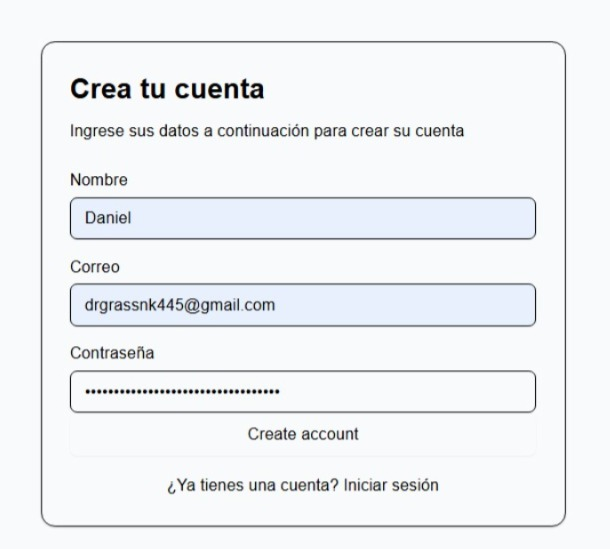
\includegraphics[width=0.6\textwidth]{images/create.jpeg} % 
		\end{center}
		\medskip % Espacio después de la imagen
	}
\end{userstory}

\begin{userstory}[hu:02] % Nueva HU
	\storyname{Iniciar sesión en el sistema}
	\storyuser{Usuario registrado}
	\storyiter{1} % Ajustar iteración
	\storypriority{Alta}
	\storyrisk{Bajo}
	\storypoints{1 semana} % Ajustar puntos
	\storyprogrammer{Daniel Rojas Grass}
	\storydescription{
		Como usuario registrado, quiero poder iniciar sesión utilizando mi email y contraseña, para poder acceder a mis conversaciones anteriores y utilizar el chat. (Corresponde principalmente a RF5, RF6, RF7, RF8, RF9)
		
		\textbf{Precondiciones:}
		\begin{itemize}
			\item El usuario tiene una cuenta registrada.
			\item El usuario no tiene una sesión activa.
			\item El usuario se encuentra en la página o sección de inicio de sesión.
		\end{itemize}
		
		\textbf{Flujo de acción:}
		\begin{enumerate}
			\item Usuario completa el formulario de inicio de sesión (email, contraseña).
			\item Usuario envía el formulario.
			\item El sistema valida las credenciales en el backend y genera una sesión/token.
			\item Si el login es exitoso, el usuario es redirigido a la interfaz principal del chat. Si falla, se muestra un mensaje de error.
		\end{enumerate}
	}
	\storyobservation{
		El manejo de la sesión/token en el frontend debe ser seguro.
	}
	\storyinterface{Formulario de Inicio de Sesión en React:
		\par\medskip % Añade un pequeño espacio vertical
		\begin{center} % Para centrar la imagen
			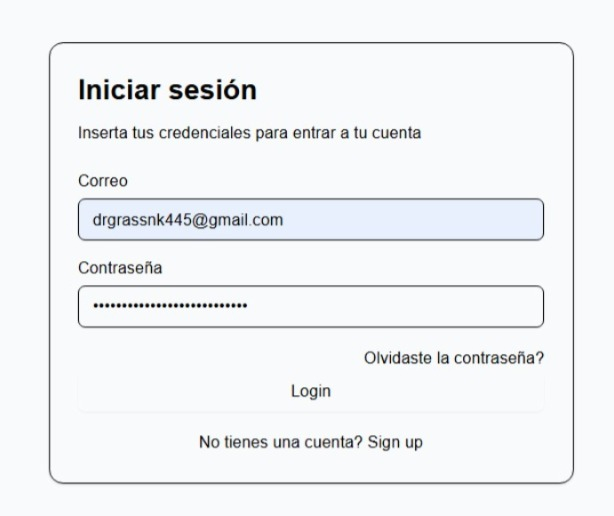
\includegraphics[width=0.6\textwidth]{images/login.jpeg} % 
		\end{center}
		\medskip
	}
\end{userstory}

\begin{userstory}[hu:03] % Nueva HU
	\storyname{Cerrar sesión del sistema}
	\storyuser{Usuario autenticado}
	\storyiter{1} % Ajustar iteración
	\storypriority{Media}
	\storyrisk{Bajo}
	\storypoints{0.5 semanas} % Ajustar puntos
	\storyprogrammer{Daniel Rojas Grass}
	\storydescription{
		Como usuario autenticado, quiero poder cerrar mi sesión activa, para asegurar que mi cuenta quede protegida al dejar de usar el sistema. (Corresponde principalmente a RF11, RF12)
		
		\textbf{Precondiciones:}
		\begin{itemize}
			\item El usuario tiene una sesión activa.
		\end{itemize}
		
		\textbf{Flujo de acción:}
		\begin{enumerate}
			\item Usuario hace clic en la opción "Cerrar Sesión".
			\item El frontend elimina el token/identificador de sesión local.
			\item (Opcional) El frontend notifica al backend para invalidar la sesión/token en el servidor.
			\item El usuario es redirigido a la página de inicio de sesión o a una página pública.
		\end{enumerate}
	}
	\storyobservation{
		Debe ser una acción fácilmente accesible desde la interfaz principal.
	}
	\storyinterface{Botón Cerrar Sesión en React:
		\par\medskip % Añade un pequeño espacio vertical
		\begin{center} % Para centrar la imagen
			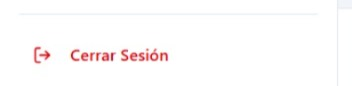
\includegraphics[width=0.6\textwidth]{images/cerrar_s.jpeg} % 
		\end{center}
	}
\end{userstory}

% ==========================================
% Gestión de Conversaciones
% ==========================================

\begin{userstory}[hu:04] % Nueva HU
	\storyname{Iniciar una nueva conversación}
	\storyuser{Usuario autenticado}
	\storyiter{2} % Ajustar iteración
	\storypriority{Alta}
	\storyrisk{Bajo}
	\storypoints{0.5 semanas} % Ajustar puntos
	\storyprogrammer{Daniel Rojas Grass}
	\storydescription{
		Como usuario autenticado, quiero poder iniciar una nueva conversación de chat, para poder realizar consultas sobre un tema nuevo sin mezclarlo con diálogos anteriores. (Corresponde principalmente a RF5)
		
		\textbf{Precondiciones:}
		\begin{itemize}
			\item El usuario tiene una sesión activa.
		\end{itemize}
		
		\textbf{Flujo de acción:}
		\begin{enumerate}
			\item Usuario hace clic en la opción "Nueva Conversación" (o similar).
			\item La interfaz de chat principal se limpia o se presenta una nueva interfaz vacía.
			\item El sistema (backend) está listo para asociar las siguientes consultas a una nueva conversación en el historial.
		\end{enumerate}
	}
	\storyobservation{
		La acción debe ser clara y resultar en una interfaz lista para una nueva interacción.
	}
	\storyinterface{Botón Nueva Conversación en React:
		\par\medskip % Añade un pequeño espacio vertical
		\begin{center} % Para centrar la imagen
			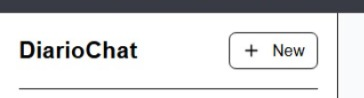
\includegraphics[width=0.6\textwidth]{images/new_c.jpeg} % 
		\end{center}
		\medskip
	}
\end{userstory}

\begin{userstory}[hu:05] % Nueva HU
	\storyname{Ver historial de conversaciones}
	\storyuser{Usuario autenticado}
	\storyiter{2} % Ajustar iteración
	\storypriority{Media}
	\storyrisk{Bajo}
	\storypoints{1 semana} % Ajustar puntos
	\storyprogrammer{Daniel Rojas Grass}
	\storydescription{
		Como usuario autenticado, quiero poder ver una lista de mis conversaciones anteriores (e.g., con títulos o fechas), para poder localizar y seleccionar una para revisión o continuación. (Corresponde principalmente a RF6)
		
		\textbf{Precondiciones:}
		\begin{itemize}
			\item El usuario tiene una sesión activa.
			\item El usuario ha tenido conversaciones previas (opcionalmente).
		\end{itemize}
		
		\textbf{Flujo de acción:}
		\begin{enumerate}
			\item Usuario accede a la sección o panel de historial.
			\item El frontend solicita la lista de conversaciones al backend.
			\item El backend recupera y envía la lista asociada al usuario.
			\item El frontend muestra la lista de conversaciones en la interfaz.
		\end{enumerate}
	}
	\storyobservation{
		La lista debe ser fácil de navegar. Considerar cómo generar títulos/identificadores útiles para cada conversación.
	}
	\storyinterface{Panel/Sección de Historial en React:
		\par\medskip % Añade un pequeño espacio vertical
		\begin{center} % Para centrar la imagen
			
\includegraphics[width=0.4\textwidth]{images/histo.jpeg} % 
		\end{center}
		\medskip
	}
\end{userstory}

\begin{userstory}[hu:06] % Nueva HU
	\storyname{Abrir una conversación del historial}
	\storyuser{Usuario autenticado}
	\storyiter{2} % Ajustar iteración
	\storypriority{Media}
	\storyrisk{Bajo}
	\storypoints{1 semana} % Ajustar puntos
	\storyprogrammer{Daniel Rojas Grass}
	\storydescription{
		Como usuario autenticado, quiero poder seleccionar una conversación específica de mi historial, para poder cargarla en la interfaz principal del chat, ver el diálogo completo y, si lo deseo, continuarla. (Corresponde principalmente a RF7)
		
		\textbf{Precondiciones:}
		\begin{itemize}
			\item El usuario tiene una sesión activa.
			\item El usuario está viendo la lista de su historial de conversaciones.
		\end{itemize}
		
		\textbf{Flujo de acción:}
		\begin{enumerate}
			\item Usuario hace clic en una conversación de la lista del historial.
			\item El frontend solicita el contenido de esa conversación al backend.
			\item El backend recupera las consultas y respuestas asociadas.
			\item El frontend carga y muestra el diálogo completo en la interfaz principal del chat.
			\item La conversación seleccionada se convierte en la conversación activa.
		\end{enumerate}
	}
	\storyobservation{
		La carga de la conversación debe ser rápida. La interfaz debe indicar claramente qué conversación está activa.
	}
	\storyinterface{Interacción con lista de Historial y Chat Principal en React:
		\par\medskip % Añade un pequeño espacio vertical
		\begin{center} % Para centrar la imagen
			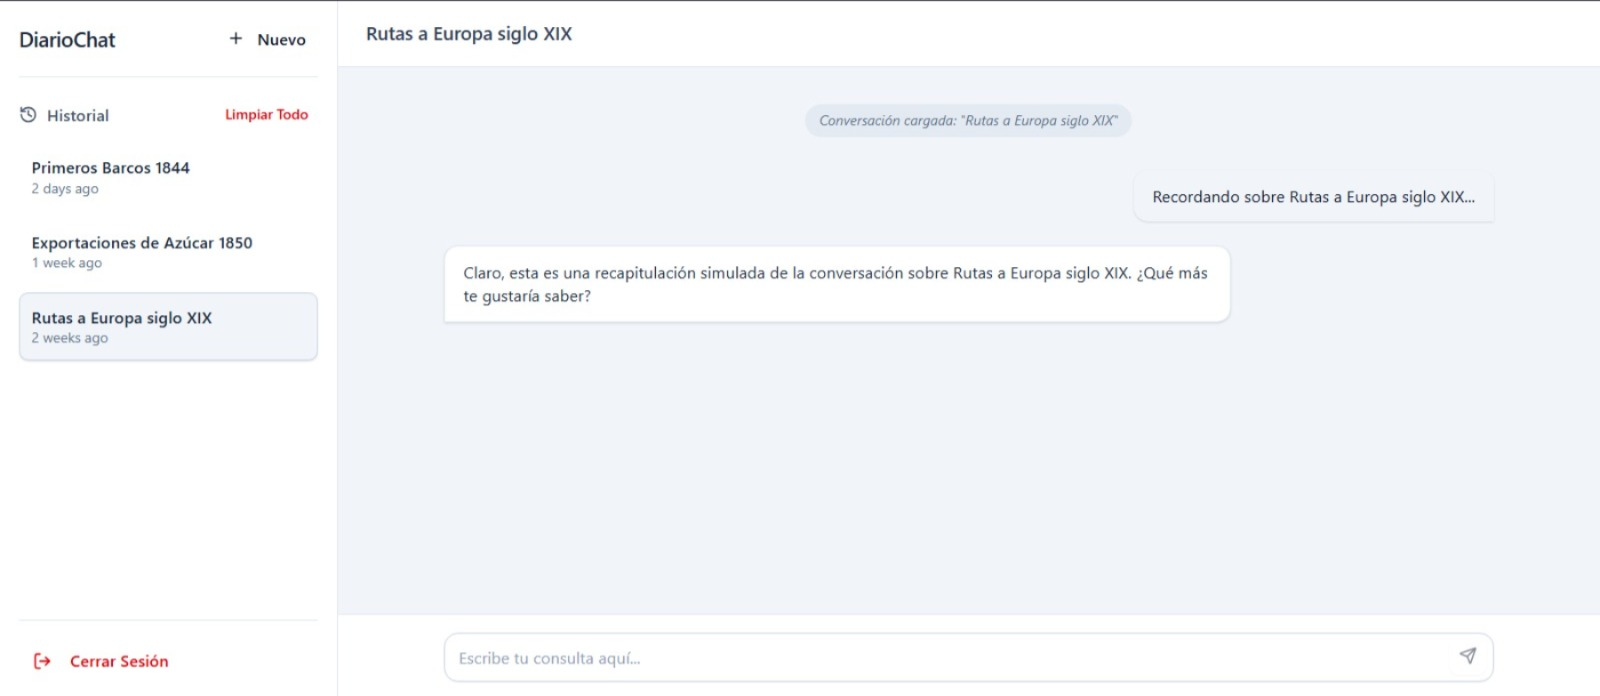
\includegraphics[width=0.6\textwidth]{images/int_ch.jpeg} % 
		\end{center}
		\medskip
	}
\end{userstory}

\begin{userstory}[hu:07] % Nueva HU
	\storyname{Eliminar una conversación del historial}
	\storyuser{Usuario autenticado}
	\storyiter{3} % Ajustar iteración
	\storypriority{Baja}
	\storyrisk{Bajo}
	\storypoints{1 semana} % Ajustar puntos
	\storyprogrammer{Daniel Rojas Grass}
	\storydescription{
		Como usuario autenticado, quiero poder eliminar una conversación específica de mi historial, para que ya no aparezca en mi lista y sus datos sean borrados permanentemente. (Corresponde principalmente a RF8)
		
		\textbf{Precondiciones:}
		\begin{itemize}
			\item El usuario tiene una sesión activa.
			\item El usuario está viendo la lista de su historial o una conversación específica.
		\end{itemize}
		
		\textbf{Flujo de acción:}
		\begin{enumerate}
			\item Usuario selecciona la opción de eliminar para una conversación específica.
			\item El sistema pide confirmación al usuario.
			\item Si el usuario confirma, el frontend envía la solicitud de eliminación al backend.
			\item El backend elimina los datos de la conversación asociada al usuario.
			\item La conversación eliminada desaparece de la lista del historial en el frontend.
		\end{enumerate}
	}
	\storyobservation{
		La eliminación debe requerir confirmación para evitar borrados accidentales.
	}
	\storyinterface{Opción de Eliminar en la lista de Historial:
		\par\medskip % Añade un pequeño espacio vertical
		\begin{center} % Para centrar la imagen
			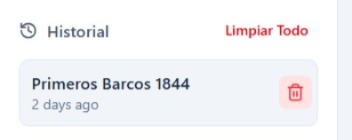
\includegraphics[width=0.6\textwidth]{images/delete_c.jpeg} % 
		\end{center}
		\medskip
	}
\end{userstory}


% ==========================================
% Funcionalidad Principal del Chat y MAS (Adaptadas y Re-numeradas)
% ==========================================

\begin{userstory}[hu:08] % Adaptada de HU:01 original
	\storyname{Interactuar con el chat activo}
	\storyuser{Usuario autenticado}
	\storyiter{1} % Mantenida
	\storypriority{Alta}
	\storyrisk{Bajo}
	\storypoints{1 semana} % Mantenido
	\storyprogrammer{Daniel Rojas Grass}
	\storydescription{
		Como usuario autenticado, quiero poder escribir consultas en lenguaje natural en la interfaz de chat activa (React), enviarlas al sistema, ver las respuestas del sistema (texto y/o imágenes) y limpiar visualmente el contenido del chat actual si lo deseo. (Corresponde principalmente a RF10, RF11, RF12, RF13)
		
		\textbf{Precondiciones:}
		\begin{itemize}
			\item El usuario tiene una sesión activa.
			\item El usuario tiene una conversación activa (nueva o cargada del historial).
		\end{itemize}
		
		\textbf{Flujo de acción:}
		\begin{enumerate}
			\item Usuario ingresa una consulta en el campo de texto del chat.
			\item Usuario envía la consulta (e.g., presionando Enter o un botón Enviar).
			\item El frontend envía la consulta al backend.
			\item El backend procesa y obtiene una respuesta (interactuando con el MAS).
			\item El backend envía la respuesta al frontend.
			\item El frontend muestra la consulta del usuario y la respuesta del sistema en el área de diálogo.
			\item (Opcional) Usuario hace clic en "Limpiar Chat" y el contenido visual del chat actual se borra.
		\end{enumerate}
	}
	\storyobservation{
		La interfaz debe ser responsiva. La presentación del diálogo (usuario/sistema) debe ser clara. Limpiar el chat no debe eliminarlo del historial.
	}
	\storyinterface{Interfaz principal del Chat en React:
		\par\medskip % Añade un pequeño espacio vertical
		\begin{center} % Para centrar la imagen
			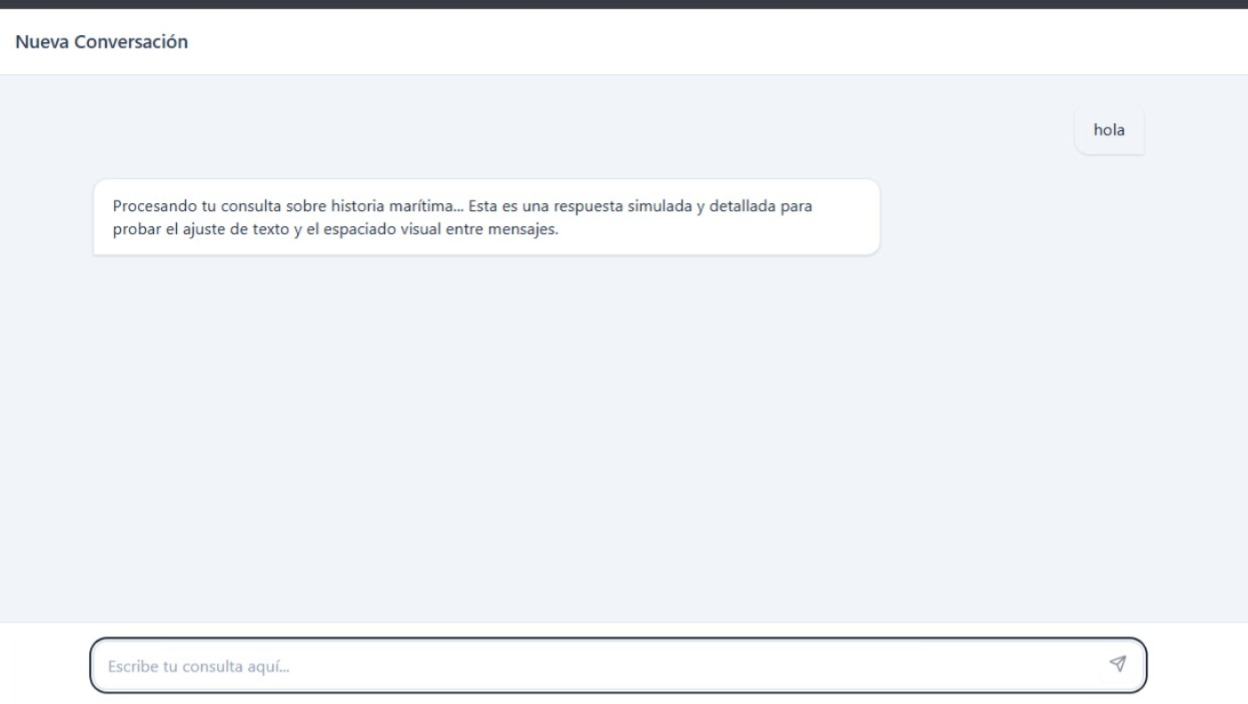
\includegraphics[width=0.6\textwidth]{images/chat.jpeg} % 
		\end{center}
		\medskip
	}
\end{userstory}

\begin{userstory}[hu:09] % Adaptada de HU:02, HU:03, HU:04, HU:06 - Enfocada en el resultado del procesamiento
	\storyname{Obtener respuesta relevante a consulta histórica}
	\storyuser{Usuario autenticado}
	\storyiter{2} % Agrupa varias iteraciones originales
	\storypriority{Alta}
	\storyrisk{Moderado} % Riesgo combinado
	\storypoints{4 semanas} % Puntos combinados (ajustar)
	\storyprogrammer{Daniel Rojas Grass}
	\storydescription{
		Como usuario autenticado, quiero que al enviar una consulta sobre el transporte marítimo del Diario de la Marina, el sistema la procese utilizando el microservicio MAS para comprenderla, buscar información relevante en los datos históricos, contextualizarla adecuadamente y validar su coherencia, para recibir una respuesta precisa y útil. (Corresponde principalmente al flujo interno del MAS: RF17 a RF29)
		
		\textbf{Precondiciones:}
		\begin{itemize}
			\item El usuario ha enviado una consulta válida desde el chat activo (HU:08).
			\item El backend ha delegado la consulta al microservicio MAS.
			\item El microservicio MAS y sus componentes (agentes, BD vectorial, LLM) están operativos.
		\end{itemize}
		
		\textbf{Flujo de acción (interno del MAS):}
		\begin{enumerate}
			\item MAS recibe la consulta.
			\item Agente Moderador analiza (palabras clave, intención).
			\item Agente Recuperador busca información en BD vectorial.
			\item Agente Contextualizador sintetiza respuesta textual y determina si se necesitan gráficos.
			\item (Si aplica) Agente Python genera y valida la imagen del gráfico.
			\item (Si aplica) Se integra texto e imagen.
			\item Agente Validación verifica coherencia y precisión.
			\item Agente Moderador ensambla la respuesta final para la API del MAS.
		\end{enumerate}
	}
	\storyobservation{
		La relevancia de la información recuperada es clave. La contextualización debe ser históricamente apropiada. La validación debe minimizar errores o "alucinaciones". La latencia del MAS es importante (ver RNF).
	}
	\storyinterface{[N/A - Proceso interno del MAS]}
\end{userstory}


\begin{userstory}[hu:10] % Adaptada de HU:05 - Enfocada en el resultado
	\storyname{Recibir visualización gráfica cuando sea pertinente}
	\storyuser{Usuario autenticado}
	\storyiter{3} % Ajustar iteración (puede ser parte de la 2)
	\storypriority{Media}
	\storyrisk{Moderado}
	\storypoints{2 semanas} % Ajustar puntos (solo la parte gráfica)
	\storyprogrammer{Daniel Rojas Grass}
	\storydescription{
		Como usuario autenticado, quiero que cuando mi consulta sugiera un análisis de patrones o tendencias (e.g., "puertos más activos en X año"), el sistema genere y me presente una visualización gráfica (e.g., gráfico de barras, mapa) junto con la respuesta textual, para facilitar la comprensión de los datos. (Corresponde principalmente a RF22, RF23, RF24, RF25, RF26)
		
		\textbf{Precondiciones:}
		\begin{itemize}
			\item El usuario ha enviado una consulta que el Agente Contextualizador interpreta como necesitada de un gráfico (dentro de HU:09).
			\item Los datos necesarios para el gráfico están disponibles.
		\end{itemize}
		
		\textbf{Flujo de acción:}
		\begin{enumerate}
			\item El Agente Contextualizador determina la necesidad del gráfico.
			\item El Agente Python genera, valida y produce la imagen del gráfico.
			\item La imagen es integrada en la respuesta final del MAS.
			\item La respuesta (incluyendo la imagen) se envía al backend y luego al frontend.
			\item El frontend muestra la imagen del gráfico junto al texto en la interfaz de chat.
		\end{enumerate}
	}
	\storyobservation{
		Los gráficos deben ser legibles y apropiados para los datos. La generación no debe fallar catastróficamente (ver RNF).
	}
	\storyinterface{Visualización de imagen dentro del Chat en React}
\end{userstory}

% HU:07 original (Entregar respuesta final) está implícitamente cubierta
% por el flujo de HU:08 y el resultado de HU:09/HU:10. No necesita
% una historia separada si HU:08 cubre la visualización.

\section{Patrones de diseño}
\label{sec:patrones_diseno}

Los patrones de diseño de software representan soluciones probadas y estandarizadas para problemas recurrentes en el desarrollo, encapsulando mejores prácticas y promoviendo la creación de software modular, legible, flexible y robusto \cite{gavilanez2022analisis}. En el desarrollo de esta aplicación web y su microservicio asociado, se han aplicado conscientemente varios patrones para abordar los desafíos inherentes a su arquitectura distribuida y su flujo de trabajo basado en IA.

\subsection{Patrones Arquitectónicos}
\label{subsec:patrones_arquitectonicos}

Estos patrones definen la estructura general del sistema y cómo sus componentes principales interactúan.

\subsubsection{Microservicios}
La arquitectura general de la solución (descrita en la Sección \ref{sec:propuesta_solucion}) adopta el patrón de \textbf{Microservicios}. El sistema se descompone en componentes independientes con responsabilidades claras: el frontend (React), el backend API (Django REST Framework) y el servicio de procesamiento de IA (Sistema Multiagente expuesto vía FastAPI).

\textbf{Justificación:} Esta separación permite el desarrollo, despliegue y escalado independientes de cada parte. Por ejemplo, el microservicio MAS, que es intensivo en recursos de IA, puede escalarse por separado del backend DRF, que maneja la lógica de negocio y la gestión de usuarios/conversaciones. Además, facilita el uso de tecnologías más adecuadas para cada tarea (React para UI, DRF para API web robusta, FastAPI/Langchain para el MAS).

\subsection{Patrones de Comportamiento}
\label{subsec:patrones_comportamiento}
Estos patrones se centran en la comunicación efectiva y la asignación de responsabilidades entre objetos/componentes.

\subsubsection{Strategy (Estrategia)}
Dentro del microservicio MAS, específicamente en el \textbf{Agente Contextualizador}, se aplica el patrón Strategy. Dependiendo de la intención identificada de la consulta del usuario (e.g., solicitud de información simple vs. solicitud de análisis que requiere visualización), el agente selecciona una estrategia diferente para construir la respuesta final.

\textbf{Justificación:} Una estrategia podría ser simplemente formatear el texto recuperado y enriquecerlo, mientras que otra estrategia implicaría coordinarse con el Agente Python para generar un gráfico e integrarlo en la respuesta. Esto permite añadir o modificar formas de responder a diferentes intenciones sin alterar la lógica principal del agente contextualizador, simplemente implementando nuevas estrategias.

\subsection{Patrones Estructurales}
\label{subsec:patrones_estructurales}
Estos patrones se ocupan de cómo se componen las clases y los objetos para formar estructuras más grandes y flexibles.

\subsubsection{Facade (Fachada)}
La \textbf{API del microservicio MAS (construida con FastAPI)} actúa como una Fachada para el complejo sistema multiagente interno. El backend DRF interactúa únicamente con esta API simplificada (e.g., un endpoint `/query`) sin necesidad de conocer los detalles de la coordinación entre los agentes (Moderador, Recuperador, Contextualizador, etc.), el acceso a la base de datos vectorial o las llamadas al LLM.

\textbf{Justificación:} Este patrón simplifica la interacción entre el backend DRF y el microservicio MAS. Reduce el acoplamiento, ya que los cambios en la lógica interna del MAS no afectan al DRF siempre que la interfaz de la API (la fachada) se mantenga estable.

\subsection{Patrones de Concurrencia}
\label{subsec:patrones_concurrencia}
Estos patrones abordan problemas relacionados con la ejecución simultánea de tareas para mejorar el rendimiento y la capacidad de respuesta.

\subsubsection{Invocación Asíncrona}
La comunicación entre los diferentes componentes de la arquitectura (Frontend $\leftrightarrow$ Backend, Backend $\leftrightarrow$ Microservicio MAS) y potencialmente dentro del MAS (llamadas a LLMs externos) utiliza invocaciones asíncronas. Por ejemplo, cuando el backend DRF llama a la API del microservicio MAS, no espera bloqueado, sino que utiliza mecanismos `async/await` (propios de frameworks como DRF/FastAPI si se configuran así) o maneja la respuesta cuando esté disponible.

\textbf{Justificación:} Esto evita que los componentes se bloqueen mientras esperan respuestas de red o tareas largas (como el procesamiento de IA), mejorando la capacidad de respuesta general del sistema y permitiendo un uso más eficiente de los recursos del servidor, ya que puede manejar otras solicitudes mientras espera. Frameworks como FastAPI están diseñados específicamente para facilitar este patrón.


\section{Targetas CRC}

Las tarjetas CRC (Clase-Responsabilidad-Colaboración) son una herramienta de diseño de software orientado a objetos, creada por Kent Beck y Ward Cunningham. Estas tarjetas se utilizan para identificar las clases, sus responsabilidades y cómo colaboran con otras clases para cumplir tareas específicas en un sistema \cite{BeckCunningham}. La representación del sistema multiagente mediante tarjetas CRC permite estructurar de forma clara y concisa las clases que lo componen, sus responsabilidades específicas y las colaboraciones necesarias para cumplir sus objetivos. Esta técnica facilita la comprensión del comportamiento de cada agente dentro del sistema —como el coordinador, el buscador de información o el generador de respuestas—, promoviendo un diseño orientado a objetos coherente, reutilizable y fácil de mantener. Además, al emplearse en etapas tempranas del desarrollo, las tarjetas CRC fortalecen la comunicación entre desarrolladores y respaldan la validación del modelo antes de su implementación definitiva.

\begin{longtable}{|l|l|}
	\caption{Tarjeta CRC: ModeratorAgent} \label{tablacrc1} \\
	
	\hline
	\multicolumn{2}{|c|}{\textbf{Tarjeta CRC}} \\
	\hline
	\textbf{Clase} & \textbf{ModeratorAgent} \\
	\hline
	\endfirsthead
	
	\hline
	\textbf{Responsabilidad} & \textbf{Colaboración} \\
	\hline
	\endhead
	
	\hline
	\multicolumn{2}{|r|}{Continúa en la próxima página} \\
	\hline
	\endfoot
	
	\hline
	\endlastfoot
	
	\parbox[t]{0.45\linewidth}{\textbf{Responsabilidades:} \\ 
		Recibir la consulta del usuario \\ 
		Extraer palabras clave e identificar la intención \\ 
		Coordinar el flujo de información entre agentes \\ 
		Ensamblar y entregar la respuesta final al usuario} 
	& 
	\parbox[t]{0.45\linewidth}{\textbf{Colaboración:} \\
		InformationRetrievalAgent \\ 
		ContextualizationAgent \\ 
		ValidationAgent}
\end{longtable}


\begin{longtable}{|l|l|}
	\caption{Tarjeta CRC: InformationRetrievalAgent} \label{tablacrc2} \\
	
	\hline
	\multicolumn{2}{|c|}{\textbf{Tarjeta CRC}} \\
	\hline
	\textbf{Clase} & \textbf{InformationRetrievalAgent} \\
	\hline
	\endfirsthead
	
	\hline
	\textbf{Responsabilidad} & \textbf{Colaboración} \\
	\hline
	\endhead
	
	\hline
	\multicolumn{2}{|r|}{Continúa en la próxima página} \\
	\hline
	\endfoot
	
	\hline
	\endlastfoot
	
	\parbox[t]{0.45\linewidth}{\textbf{Responsabilidades:} \\ 
		Convertir las palabras clave en embeddings \\ 
		Consultar la base de datos vectorial para recuperar la información relevante \\ 
		Devolver los resultados al ModeratorAgent} 
	& 
	\parbox[t]{0.45\linewidth}{\textbf{Colaboración:} \\
		ModeratorAgent \\ 
		FaissDatabase}
\end{longtable}

\begin{longtable}{|l|l|}
	\caption{Tarjeta CRC: ContextualizationAgent} \label{tablacrc3} \\
	
	\hline
	\multicolumn{2}{|c|}{\textbf{Tarjeta CRC}} \\
	\hline
	\textbf{Clase} & \textbf{ContextualizationAgent} \\
	\hline
	\endfirsthead
	
	\hline
	\textbf{Responsabilidad} & \textbf{Colaboración} \\
	\hline
	\endhead
	
	\hline
	\multicolumn{2}{|r|}{Continúa en la próxima página} \\
	\hline
	\endfoot
	
	\hline
	\endlastfoot
	
	\parbox[t]{0.45\linewidth}{\textbf{Responsabilidades:} \\ 
		Recibir la información relevante y la intención del usuario \\ 
		Generar indicaciones de estadísticas o contextualizar la información según la petición del usuario \\ 
		Enviar la información procesada al ModeratorAgent} 
	& 
	\parbox[t]{0.45\linewidth}{\textbf{Colaboración:} \\
		ModeratorAgent \\ 
		PythonAgent}
\end{longtable}


\begin{longtable}{|l|l|}
	\caption{Tarjeta CRC: ValidationAgent} \label{tablacrc4} \\
	
	\hline
	\multicolumn{2}{|c|}{\textbf{Tarjeta CRC}} \\
	\hline
	\textbf{Clase} & \textbf{ValidationAgent} \\
	\hline
	\endfirsthead
	
	\hline
	\textbf{Responsabilidad} & \textbf{Colaboración} \\
	\hline
	\endhead
	
	\hline
	\multicolumn{2}{|r|}{Continúa en la próxima página} \\
	\hline
	\endfoot
	
	\hline
	\endlastfoot
	
	\parbox[t]{0.45\linewidth}{\textbf{Responsabilidades:} \\ 
		Revisar la coherencia de la respuesta generada por el sistema \\ 
		Comparar la respuesta con la entrada original \\ 
		Validar o rechazar la respuesta antes de enviarla al usuario} 
	& 
	\parbox[t]{0.45\linewidth}{\textbf{Colaboración:} \\
		ModeratorAgent \\ 
		ContextualizationAgent}
\end{longtable}

\begin{longtable}{|l|l|}
	\caption{Tarjeta CRC: PythonAgent} \label{tablacrc5} \\
	
	\hline
	\multicolumn{2}{|c|}{\textbf{Tarjeta CRC}} \\
	\hline
	\textbf{Clase} & \textbf{PythonAgent} \\
	\hline
	\endfirsthead
	
	\hline
	\textbf{Responsabilidad} & \textbf{Colaboración} \\
	\hline
	\endhead
	
	\hline
	\multicolumn{2}{|r|}{Continúa en la próxima página} \\
	\hline
	\endfoot
	
	\hline
	\endlastfoot
	
	\parbox[t]{0.45\linewidth}{\textbf{Responsabilidades:} \\ 
		Generar un script de Python para representar estadísticas gráficas cuando sea necesario \\ 
		Validar el script y asegurarse de que sea correcto \\ 
		Convertir el gráfico generado en una imagen que pueda ser integrada en la respuesta final} 
	& 
	\parbox[t]{0.45\linewidth}{\textbf{Colaboración:} \\
		ContextualizationAgent \\ 
		ImageGenerationTool}
\end{longtable}






\section{Diagrama de componentes}

Los diagramas de componentes son una herramienta fundamental en ingeniería de software para visualizar la organización y las relaciones entre los componentes de un sistema. Estos diagramas proporcionan una vista de alto nivel de la arquitectura del sistema, mostrando cómo los componentes interactúan a través de interfaces bien definidas. Esto es especialmente útil en sistemas complejos, donde entender las interacciones entre componentes es crucial para el diseño y la implementación efectivos \cite{Restackio2025}.

\begin{figure}[h]
	\centering
	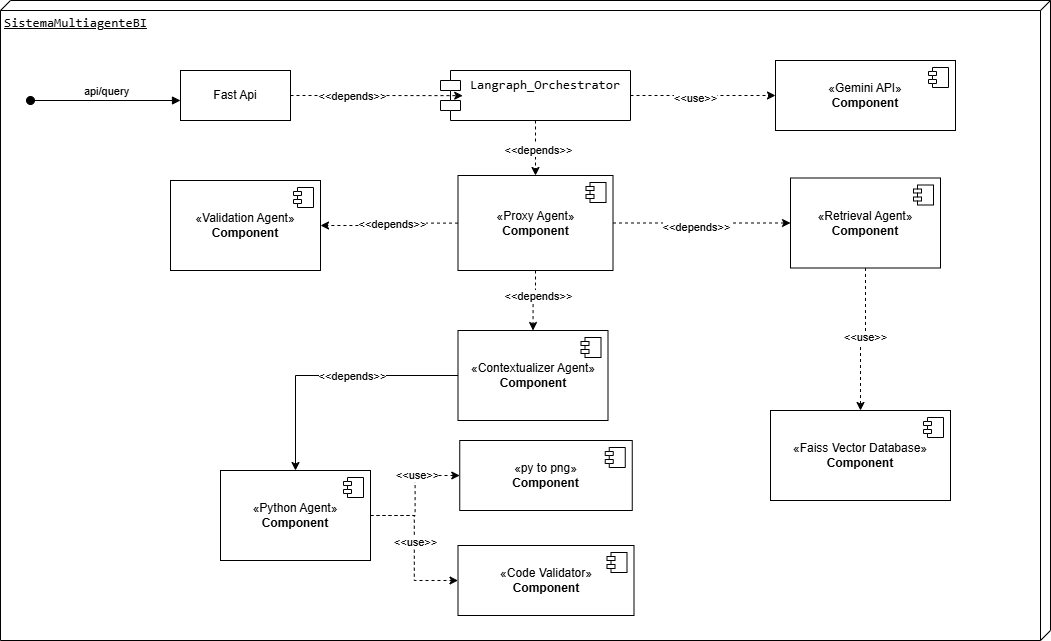
\includegraphics[width=0.7\textwidth]{images/component.png}
	\caption{Diagrama de Componentes.}
	\label{fig:Diagrama de Componente.}
\end{figure}

